% !TeX spellcheck = en_GB
% !TeX encoding = UTF-8
% !TeX root = ../report.tex

\chapter{Implementation}
\label{chp:Implementation}

\section{Implementation Hardware}
\subsection{Braking}

Braking presented itself to be the technically most difficult aspect in the drive-by-wire system. The kart offered limited space, therefore a very efficient actuator was needed to ensure the Force necessary for an emergency brake. Early testing showed that for a full brake roughly 250-350 N of force was required. However, this testing was done with the kart jacked up, therefore we could not fully rely on these results.
%brake hydraulic complicated not interfering 

Early on we set a few requirements for our brake actuator, namely speed, force and precision. After some research we decided to look further into a high end linear motor by LinMot and neglect the idea of a rotary motor. Our main reasons being that a rotary motor generally was significantly slower and usually required external sensors to be precise enough.\\
We also dismissed the intriguing concept of directly interfering with the hydraulic system, for example inserting an electro hydraulic pump into the system. Our main reasoning against this was that it would require a lot of time, effort and would most likely not outperfom a simpler mechanical brake actuator.

A very easy to implement and cost efficient method of braking that we proposed was plugging braking. The idea was to use the kart's electro motors to brake, by reversing the current. While it would not need any additional parts and would only require some programming, we soon realised the braking power generated by the hydraulic brake sufficed for a full brake and power consumption would rise significantly. \\Because time was running low and we had to decide for a reliable solution, we chose a linear motor over the plugging braking option. If we had more time on our hands and could have done some testing of the required braking power, we might have decided otherwise.

With all other options out of our way, we were now able to focus on the linear motor.
With our battery providing 48 VDC, LinMot's range of motor narrowed down quite a bit. The PS01-48x240F-C was our first idea, as it provided up to 572 N of maximum force. We quickly realized that our limited space would not allow for such a big motor. After a personal consultation with one of LinMot's employees, we decided for a PS01-37x120F-HP-C with a 300 mm runner.\\ Because of the smaller size, we now had various options of where to put the linear motor. Again, we strived for an easy installation. Therefore we determined the best location to be on top of the brake cylinder, just in between the two pedals. Pushing the pedal resulted in a slightly arc shaped downward motion of the braking lever. This is the point where the motor's runner has been attached to the lever. As the linear motor should not be under radial load, a design had to be realized which allowed the motor to tilt slightly. This helped to reduce the radial load, as the downward motion could be compensated with tilting the motor at an angle.

This notion was put into place by mounting the linear motor on a metal frame right above the braking cylinder. The frame is made of two sheets of metal connected by multiple steel linkages. The motor is held on the frame with two ball-bearings, allowing for a pitch motion and therefore preventing any major radial forces.
The metal sheets were cut by a water jet cutter.

\begin{figure}[h]
	\centering
	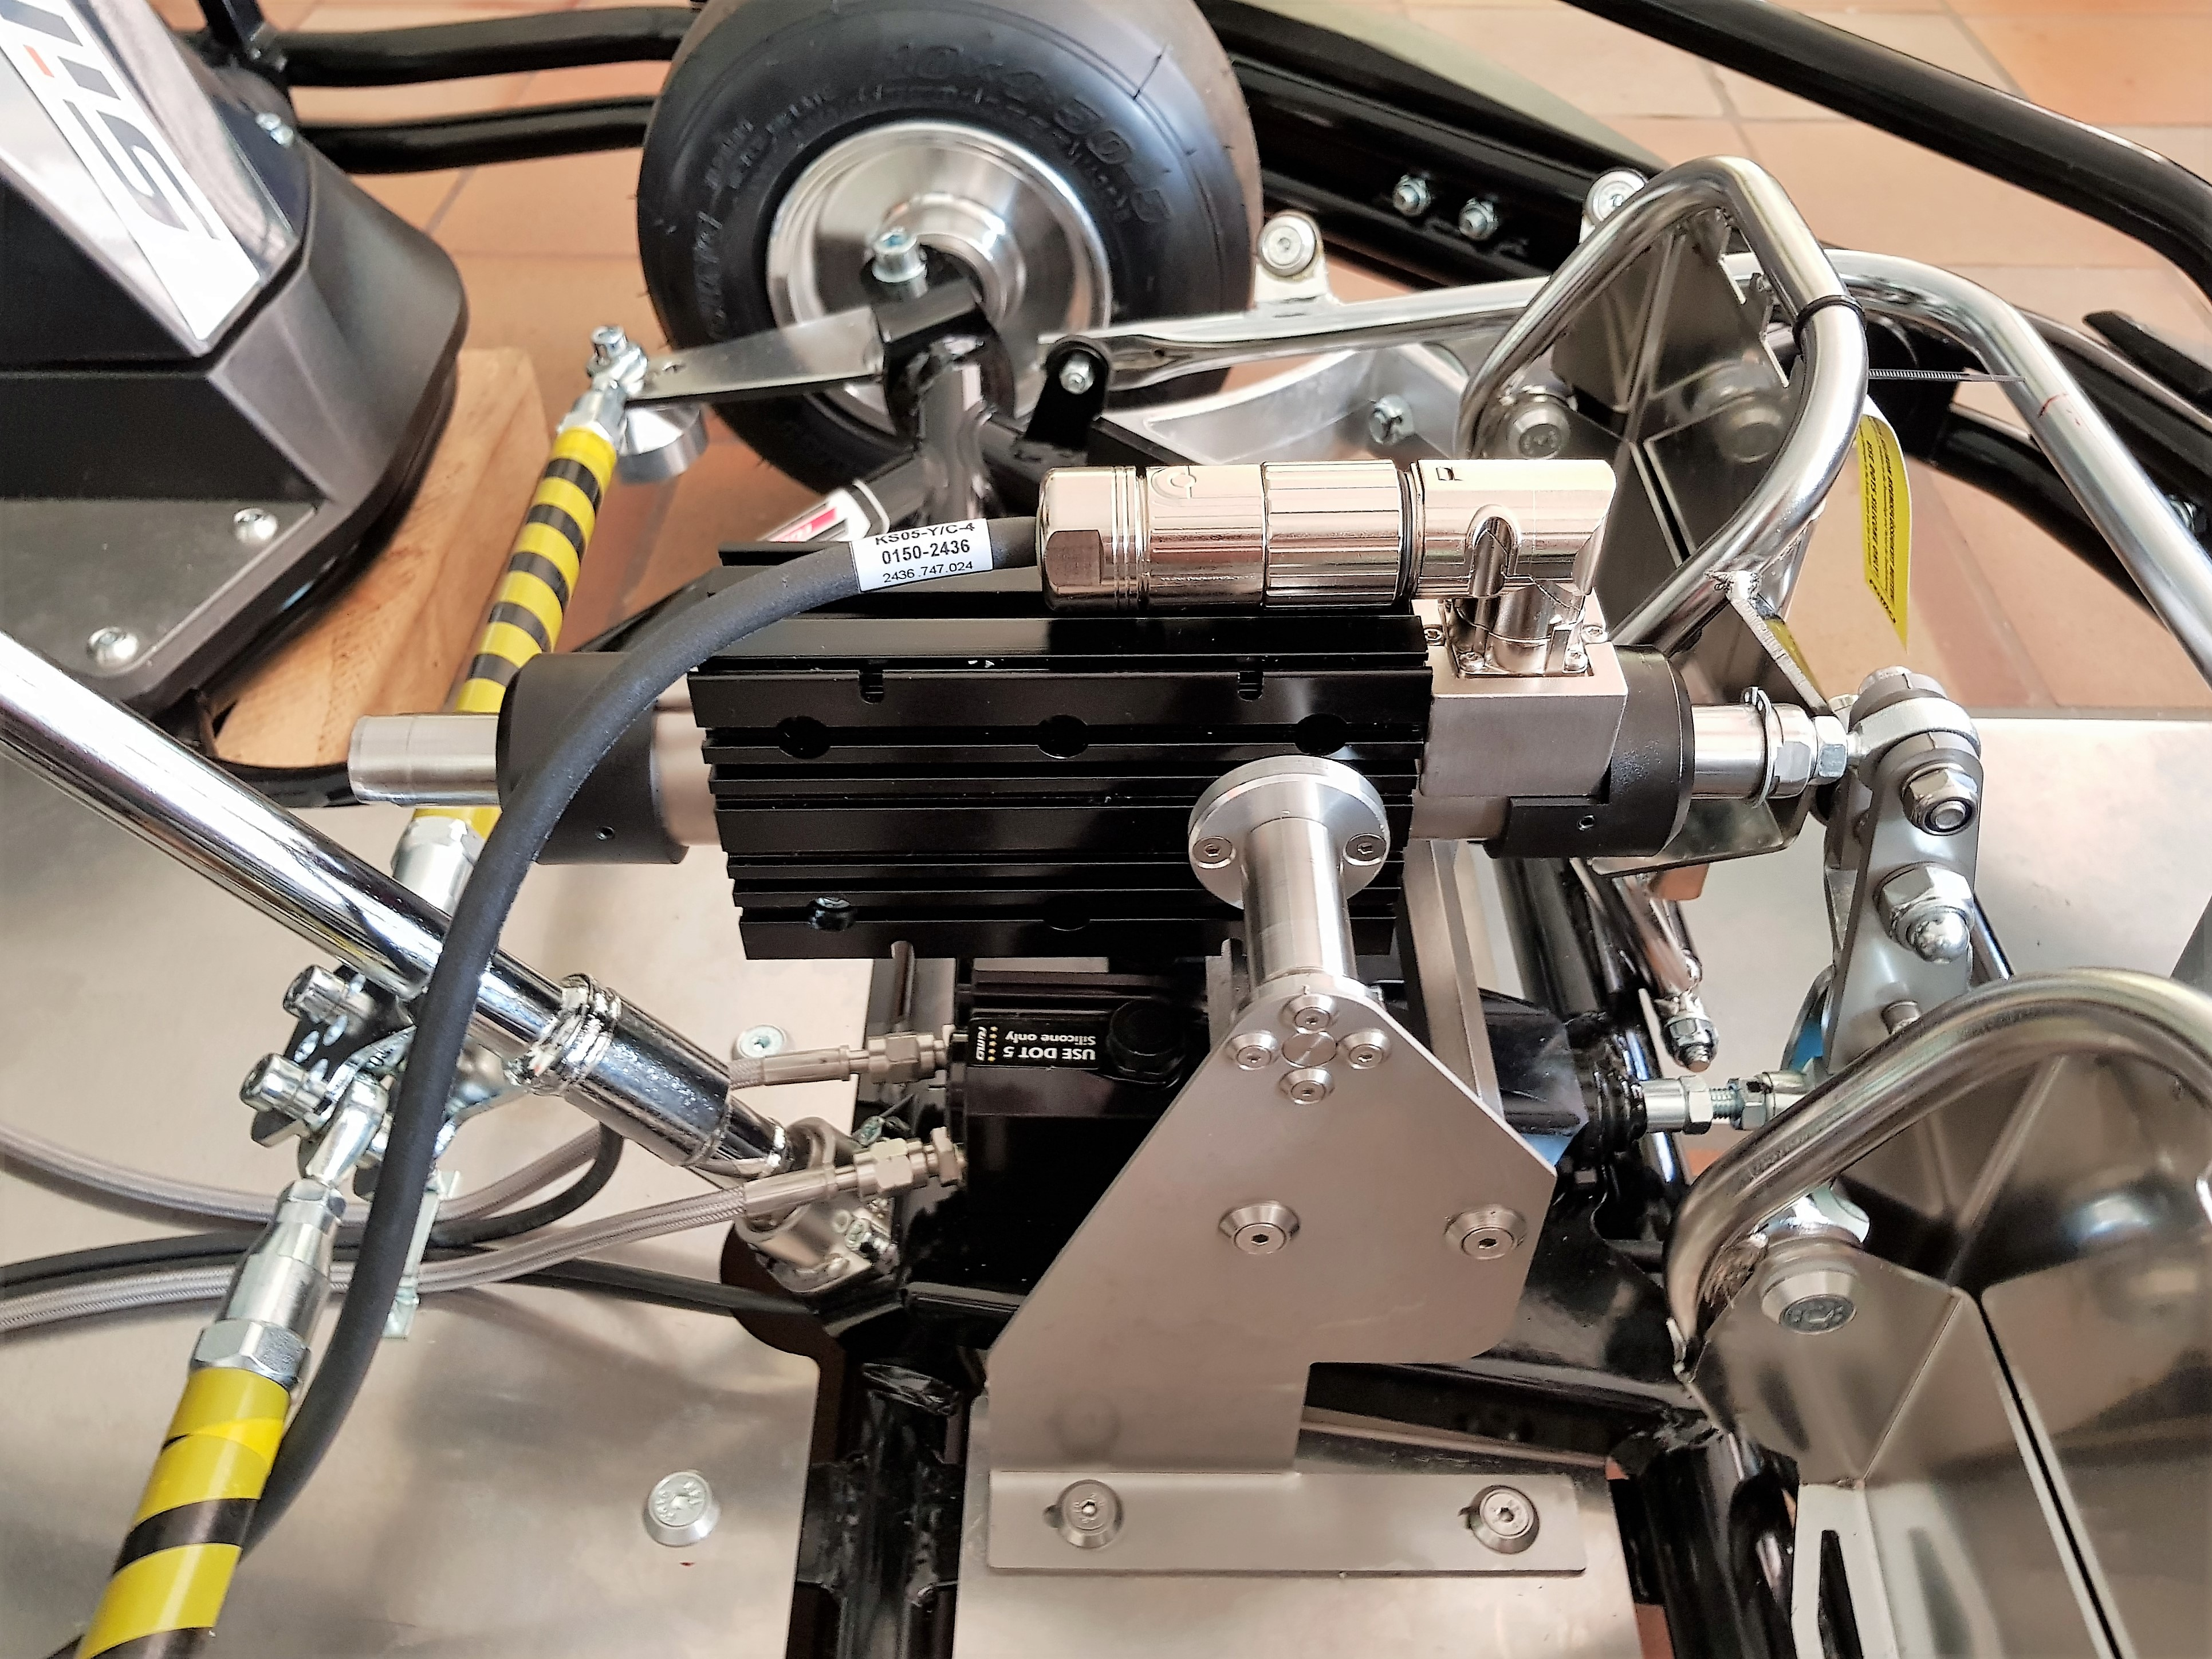
\includegraphics[width=0.7\linewidth]{pictures_figures/Used/Picture_brake}
	\caption{}
	\label{fig:picturebrake}
\end{figure}


\subsection{Throttle}

To control the throttle, we had to access the ACD 4805 motor controller of each electric drive. After a simple start up sequence, we were able to control the velocity of each wheel via CANOpen. For throttling, no actuators had to implemented. The crucial work that went into throttle-by-wire part was mainly communication and will therefore be discussed in the following chapter.

\newpage

\subsection{Steering}

As already mentioned in chapter one, we used a compact power steering unit, with a rated torque of around 3 Nm. In order to install the unit, the kart's steering column was cut up, as was the power steering's drive shaft. The column and the drive shaft were then joined together by using press-fit joints. To counter the motor's torque, we fixed it to the steering wheel's metal holder and reinforced it with an additional steel linkage.

\begin{figure}[h]
	\centering
	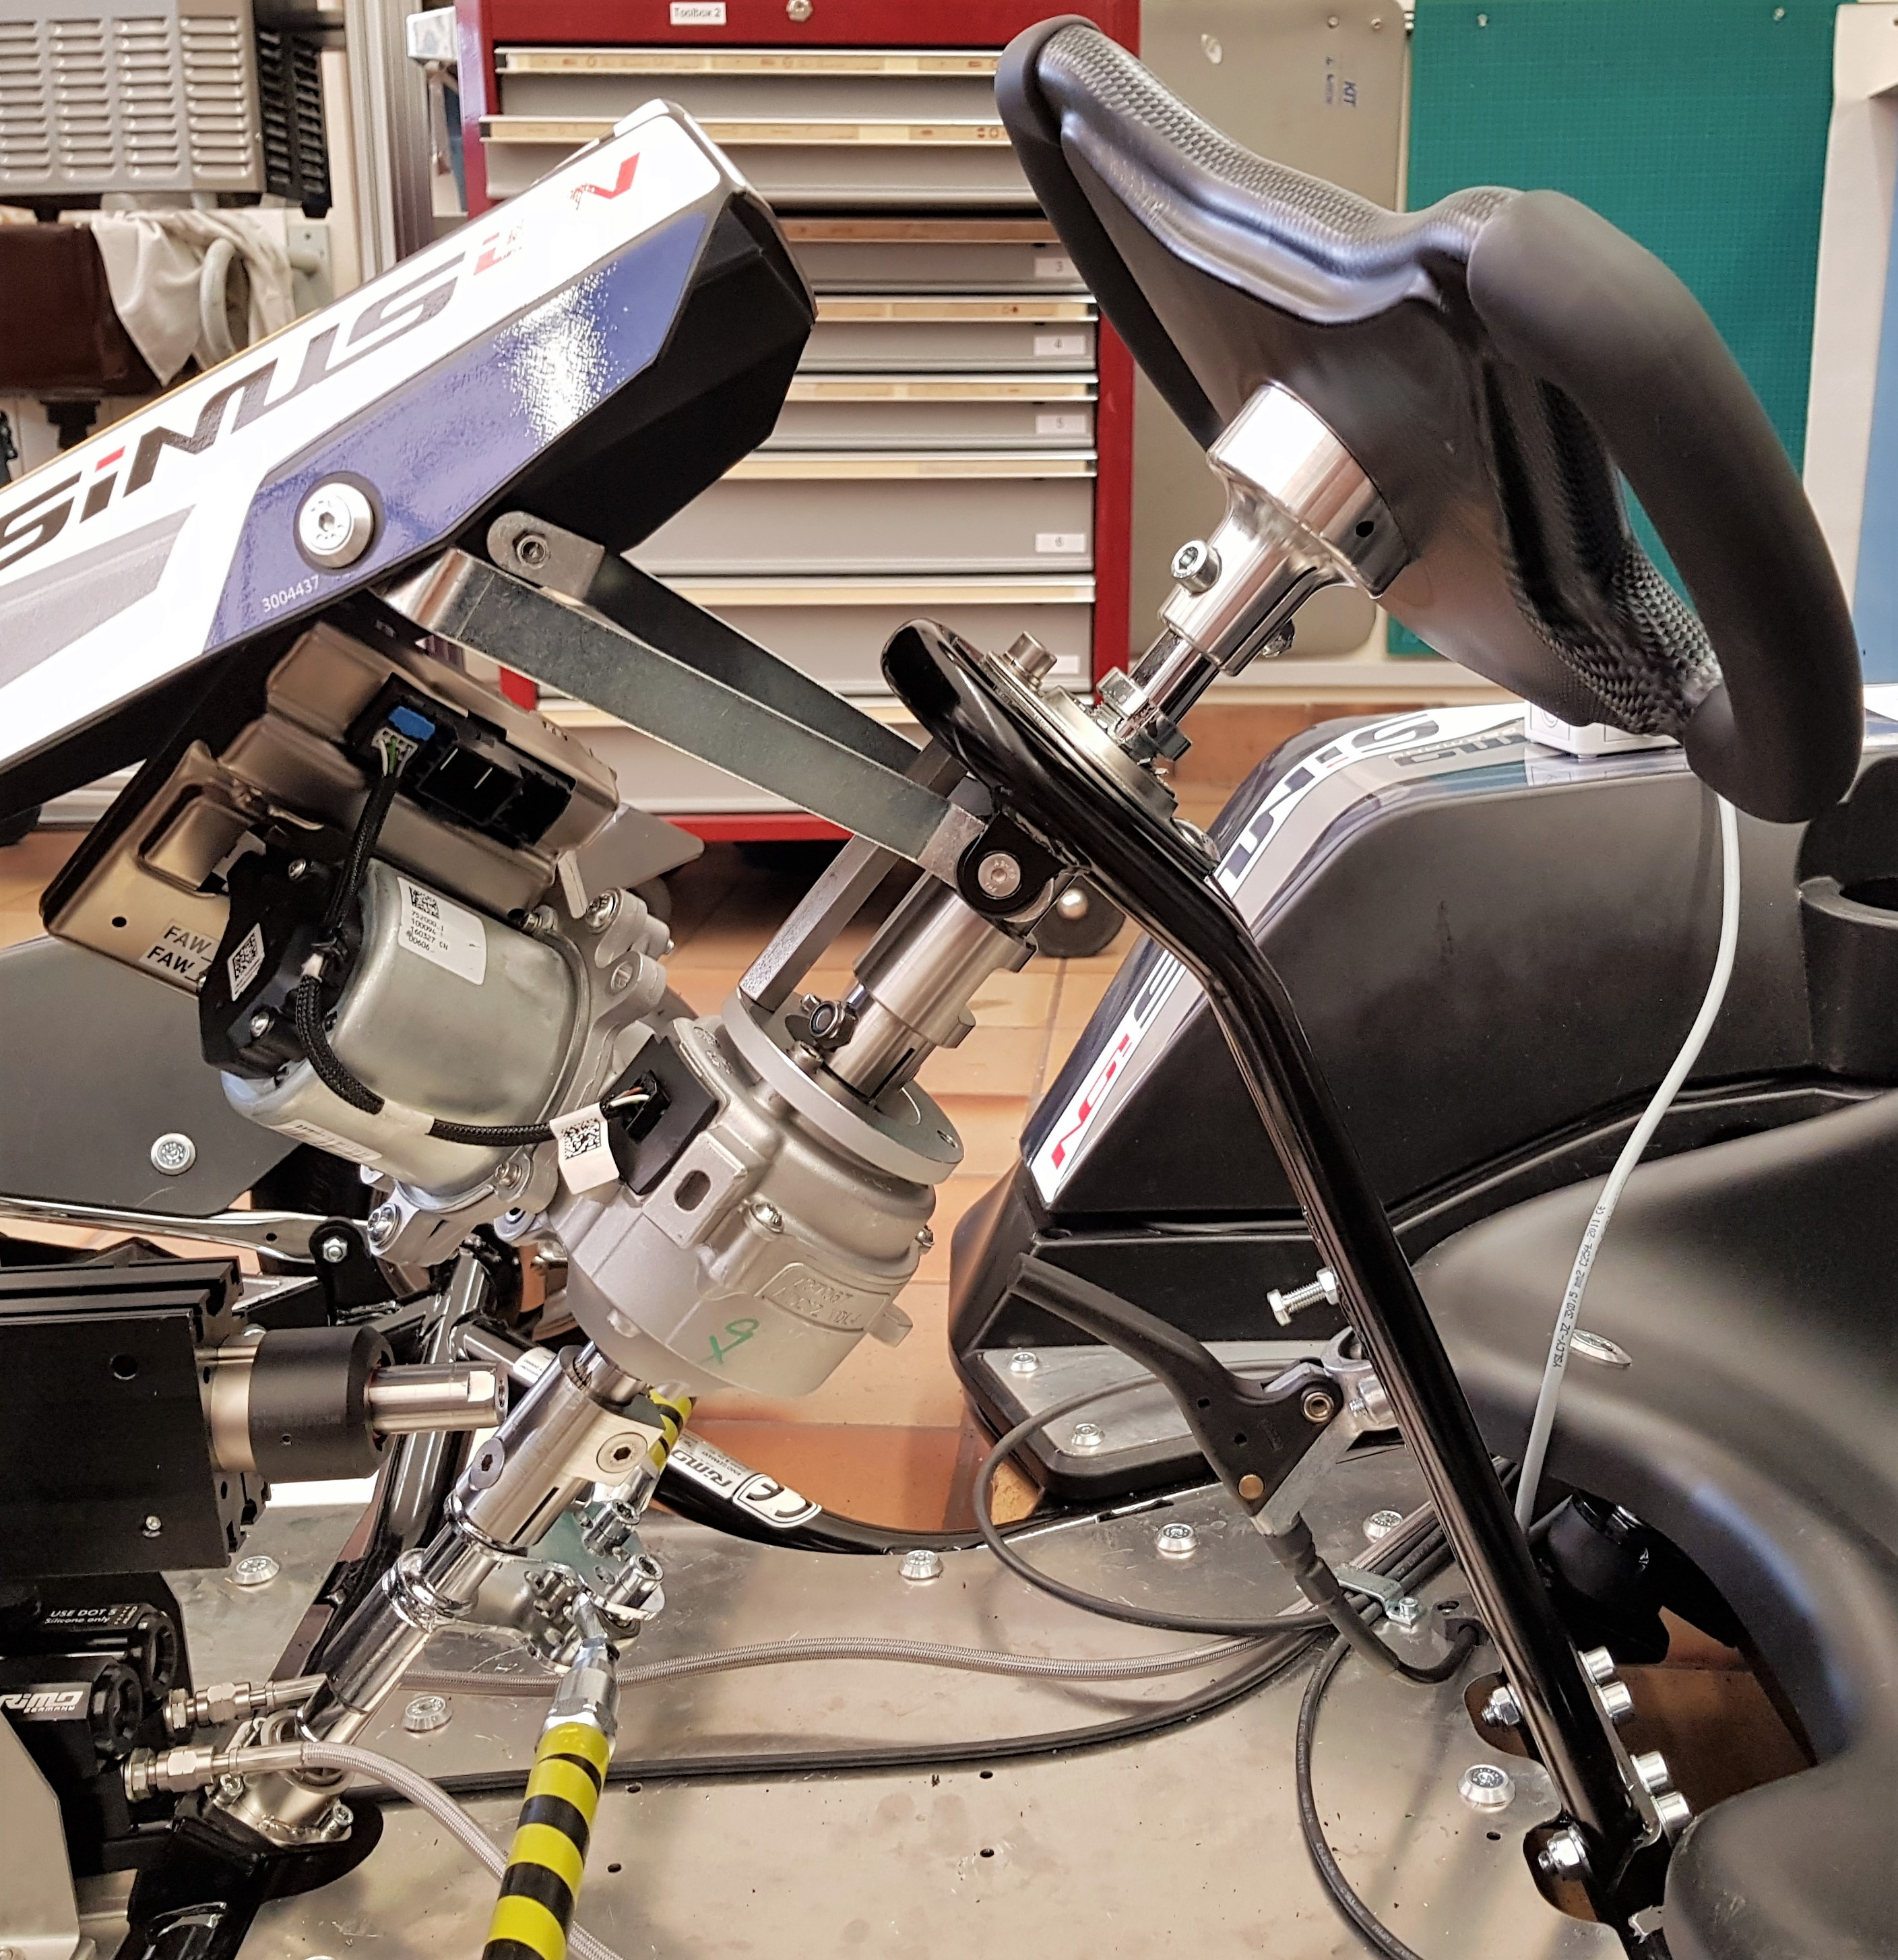
\includegraphics[width=0.7\linewidth]{pictures_figures/Used/picture_powersteering}
	\caption{}
	\label{fig:picturepowersteering}
\end{figure}

\section{Implementation Communication}

\subsection{ACD}
%explain what commands we used, object dictionary and relevant commands/messages.



%write about RPDO1 RPDO2 conflict, our assumptions what if couldve been, namely phyiscal connection, sync messages, overload, messages overlapping etc. solved by disabling rpdo2

In order to communicate with the ACD, the CAN Node-Id of each ACD had to be determined. One of Rimo's pdf files, namely "Setting up ACD Controller \& Connection Diagram", serves exactly this purpose. 
%refer to appendix witht file.
To find the respective node-id's, we had to check if either pin 12 (DI5) or pin 20 (DI6) was connected to any other pins on the ACD 4805 K1 connector. In our case, pin 12 of the right ACD was connected to pin 1, making it node 6. Pin 12 of the left ACD was not connected and therefore making it node 5. Afterwards our findings were confirmed when we connected the go-kart to our CAN bus. With the help of a CAN-USB adapter, we were able to receive and send messages, and after a while controlling the kart.
Because the go-kart does not communicate via CAN by default but only for service and remote control purposes, we had to put all nodes into operational mode by sending a NMT start messages to all nodes, namely node 5 and 6.
The ID of a NMT message is 0x000, to start the nodes the instruction code 0x01 had to be used. To reach all nodes simultaneously, the node adress needed to be 0x0. 

Issues with CANOpen and dSpace. 

When we tried to control the ACD via CANOpen with the Microautobox, the communication presented itself to be an issue. The wheels were not turning smoothly, but rather interrupted from time to time. We assumed that something had to be disrupting the communication.
With the help of a CAN-USB adapter, we were able to monitor the CAN bus. After checking all physical layers, we came to the conclusion that it must be a software problem. Our first approach was to change synchronisation times. This however did not have any effect, neither did changing the baud rate or adjusting the step size for Matlab's solver.
A smooth motion of the motors could be realized by sending the Receive PDO manually via the PCAN software. The problem turned out to arise from the second Receive PDO. While the first RPDO determines the target speed for the speed controller the second RPDO provides the possibility to control the motor with via torque control. By default, the use of one of the mentioned does not disable the function of the other. This leads to critical failure causing improper motion if both RPDOs are sent simultaneously. The motor tries to achieve both, target speed and target torgue ending up rapidly switching the motor current. The problem could be solved by completely removing the second RPDO from the Matlab model. We were not able to deactivate an individual PDO's transmission in real time with dSpace CANOpen solution.



Two's complement is convenient way to store integers, such that adding and subtracting with negative numbers becomes very easy. This was used on the ACD 4805, where certain values, such as the rotational speed of the wheels, can be negative. 
The basic principles of two's complement are the following.

- Zero is represented by all 0's. 
e.g. 0 0 0 0 = 0

- The maximum positive integer is $ 2^{number of bits-1}-1 $.
So for 4 bits, the biggest integer is therefore 0 1 1 1 = 7, and not 1 1 1 1 = 15 as in the standard notation.

- if the integer is negative, 1's and 0's switch roles, starting from all one's, e.g. 1 1 1 1 = -1. This increases the range for negative numbers by one.

So for 4 bits it looks as follows.

\begin{tabular}{llll}
	0 0 0 0 = 0 & 0 1 0 0 = 4 & 1 1 1 1 = -1 & 1 0 1 1 = -5\\
	0 0 0 1 = 1 & 0 1 0 1 = 5 & 1 1 1 0 = -2 & 1 0 1 0 = -6\\
	0 0 1 0 = 2 & 0 1 1 0 = 6 & 1 1 0 1 = -3 & 1 0 0 1 = -7\\
	0 0 1 1 = 3 & 0 1 1 1 = 7 & 1 1 0 0 = -4 & 1 0 0 0 = -8
\end{tabular}

So an easy way to find the negative integer of a positive integer is to convert the desired decimal number to binary, inverting all 0's and 1's and then adding 1. A more hands on approach is to again convert to binary, starting from the right to find the first 1 and inverting all bits to the left of it.

So in order to have a rotational speed of -500 revolutions per minute, the following steps have to be taken for a signed 16 bit integer.

500 = 0 0 0 0 \: 0 0 0 1 \: 1 1 1 1 \: 0 1 0 0

Now invert all bits.

1 1 1 1 \: 1 1 1 0 \: 0 0 0 0 \: 1 0 1 1

And add 1

1 1 1 1 \: 1 1 1 0 \: 0 0 0 0 \: 1 1 0 0 = -500

The second method would result in the following steps.

Starting from the right, find first 1.

500 = 0 0 0 0 \: 0 0 0 1 \: 1 1 1 1 \: 0 \textbf{1} 0 0

Invert all consecutive bits to the left of it.

1 1 1 1 \: 1 1 1 0 \: 0 0 0 0 \: 1 \textbf{1} 0 0 = -500

If a signed integer is postive or negative is easy to spot, as it's most significant bit determines if the number is negative or positive. 1 = negative, 0 = positive.

\subsection{LinMot}
important settings

For some reason, TPDO3 and TPDO4 would not transmit their data when a sync message was sent. This was tried to solve by setting the intern event timer to around 10 ms and changing the transmission type to 254. However, after a while it would stop transmitting out of a unknown reason. As time was scarce, we simply remapped the PDOs, such that the needed data would be transmitted via TPDO2. 

%talk about failsafe for brake

Another issues presented itself while working on the brake. Previously we used a motion command called VAI go to position 16bit, which takes velocity, acceleration/deceleration and position as input and creates a curve for the linear motor, which results in the motion. However, a new command will only be executed if the last four bits of the motion command header, called command count, has changed. In the easiest way, bit 0 can be toggled. 
To avoid this, a different setting could be utilized, called PV Stream. This uses a constant stream of position and velocity inputs during a fixed streaming period, interpolates and executes the command. While this seemed very intriguing, it's implementation was not possible. For some reason an error arose, stating that our streaming was too slow. Even after checking the period time with PCAN and checking all settings, the issue could not be resolved.
After that, we went back to the prior way of setting the position.

To counteract the need for change in the command count in order for a change in motion we introduced a pulse generator into the Matlab model.
The pulse generators output is an alternating signal either being zero or one. With the signal from the pulse generator added to the command header, the command count changes every halve period of the pulse generator. With a sufficiently low pulse generator period a function similar to the PV stream could be implemented.
%%really
%clock not working as it triggers resets all the time

\subsection{Power steering}

As of now, the needed simulink blocks for the power steering have not yet arrived. Communication is therefore not yet possible with the power steering unit and will not covered in this section.



